The lepton identification and isolation requirements significantly suppress
the background contribution, and the remnant portion of it is very small compared to the signal.
We can identify two main background components: an irreducible background from genuine four high-$p_T$ isolated leptons processes, such as $t\bar{t}Z$, $WWZ$ and $t\bar{t}WW$,  and a reducible background from processes with less than four leptons, but with jets that are misidentified as leptons. 

The irreducible background is very small and it is estimated using MC samples (see Fig.~\ref{fig:irr_bkg}).
\begin{figure}[hbtp]
  \begin{center}
   % 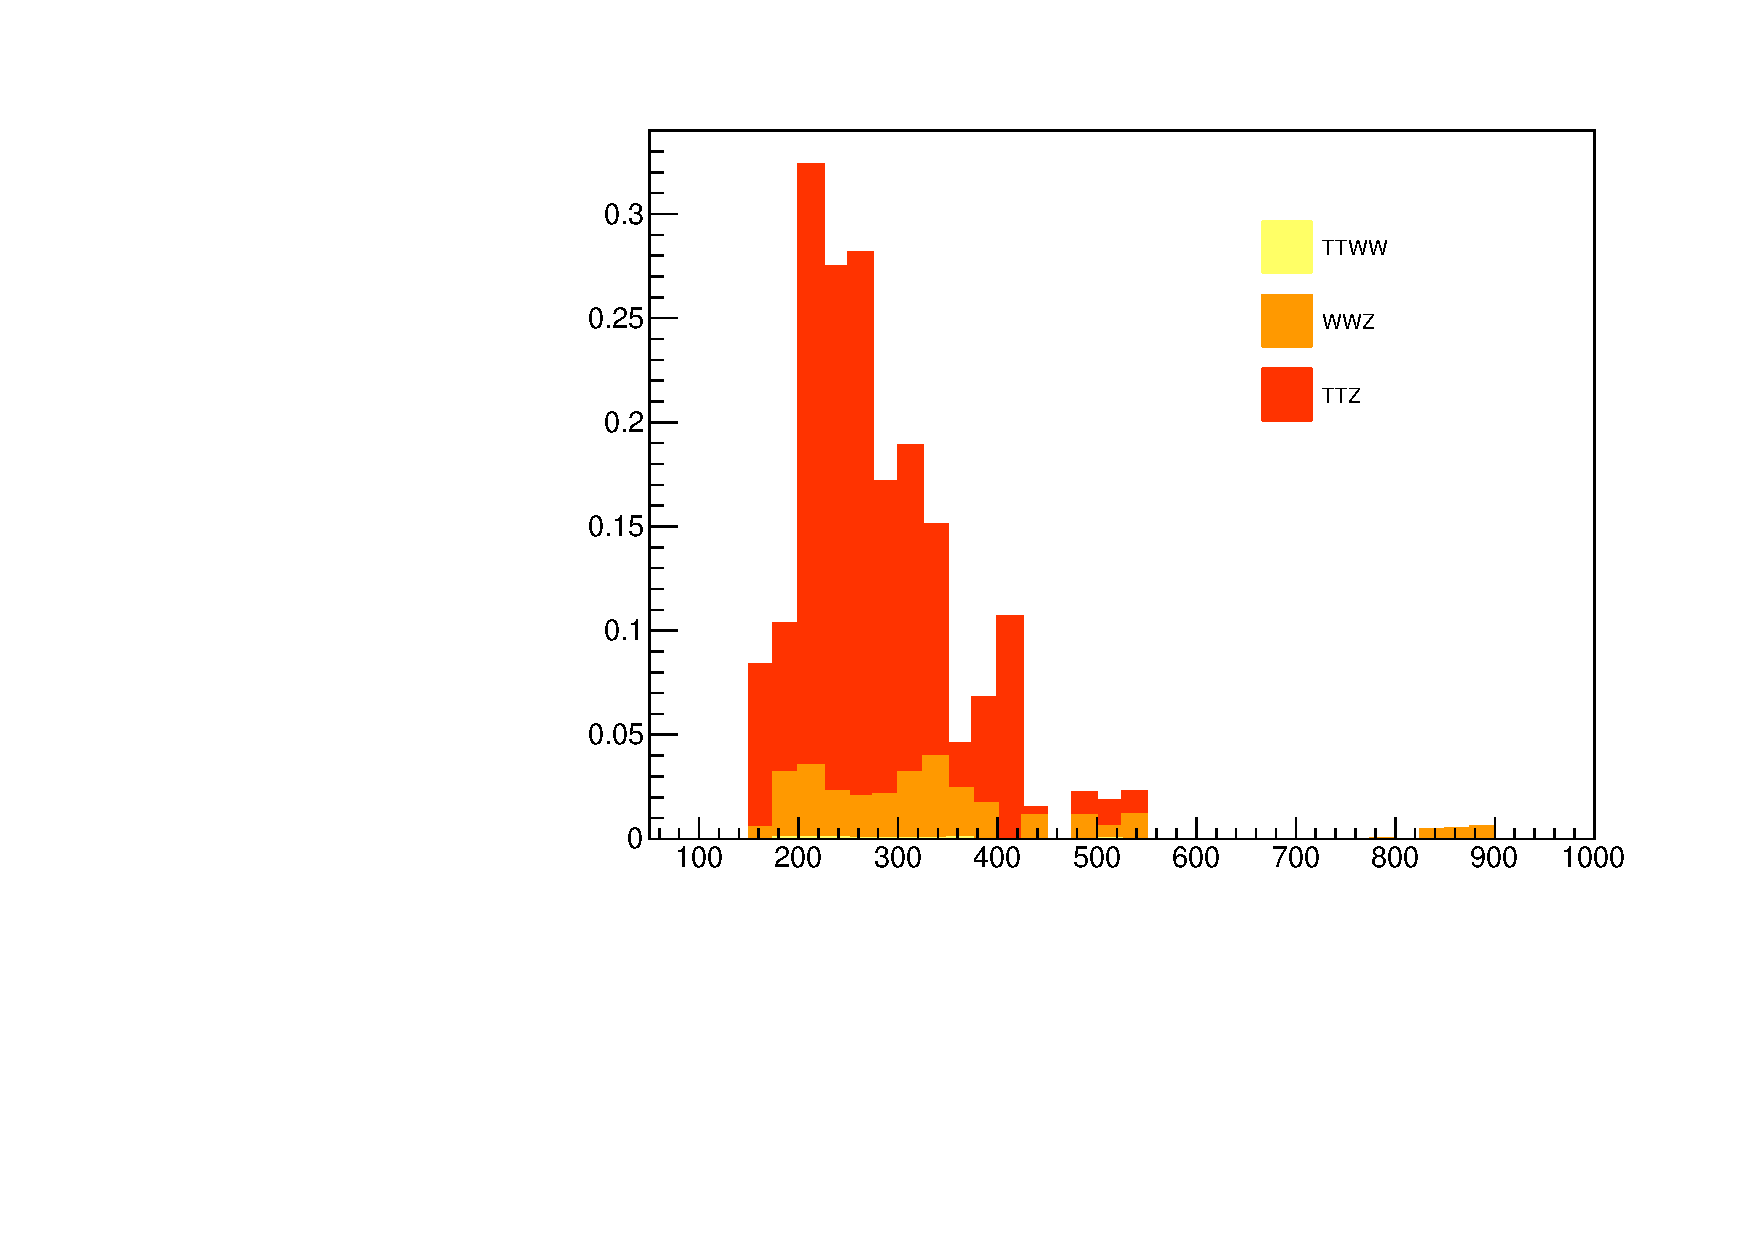
\includegraphics[width=\cmsFigWidth]{Figures/Mass_Irreducible_Bkg_MadGraphSet}
    %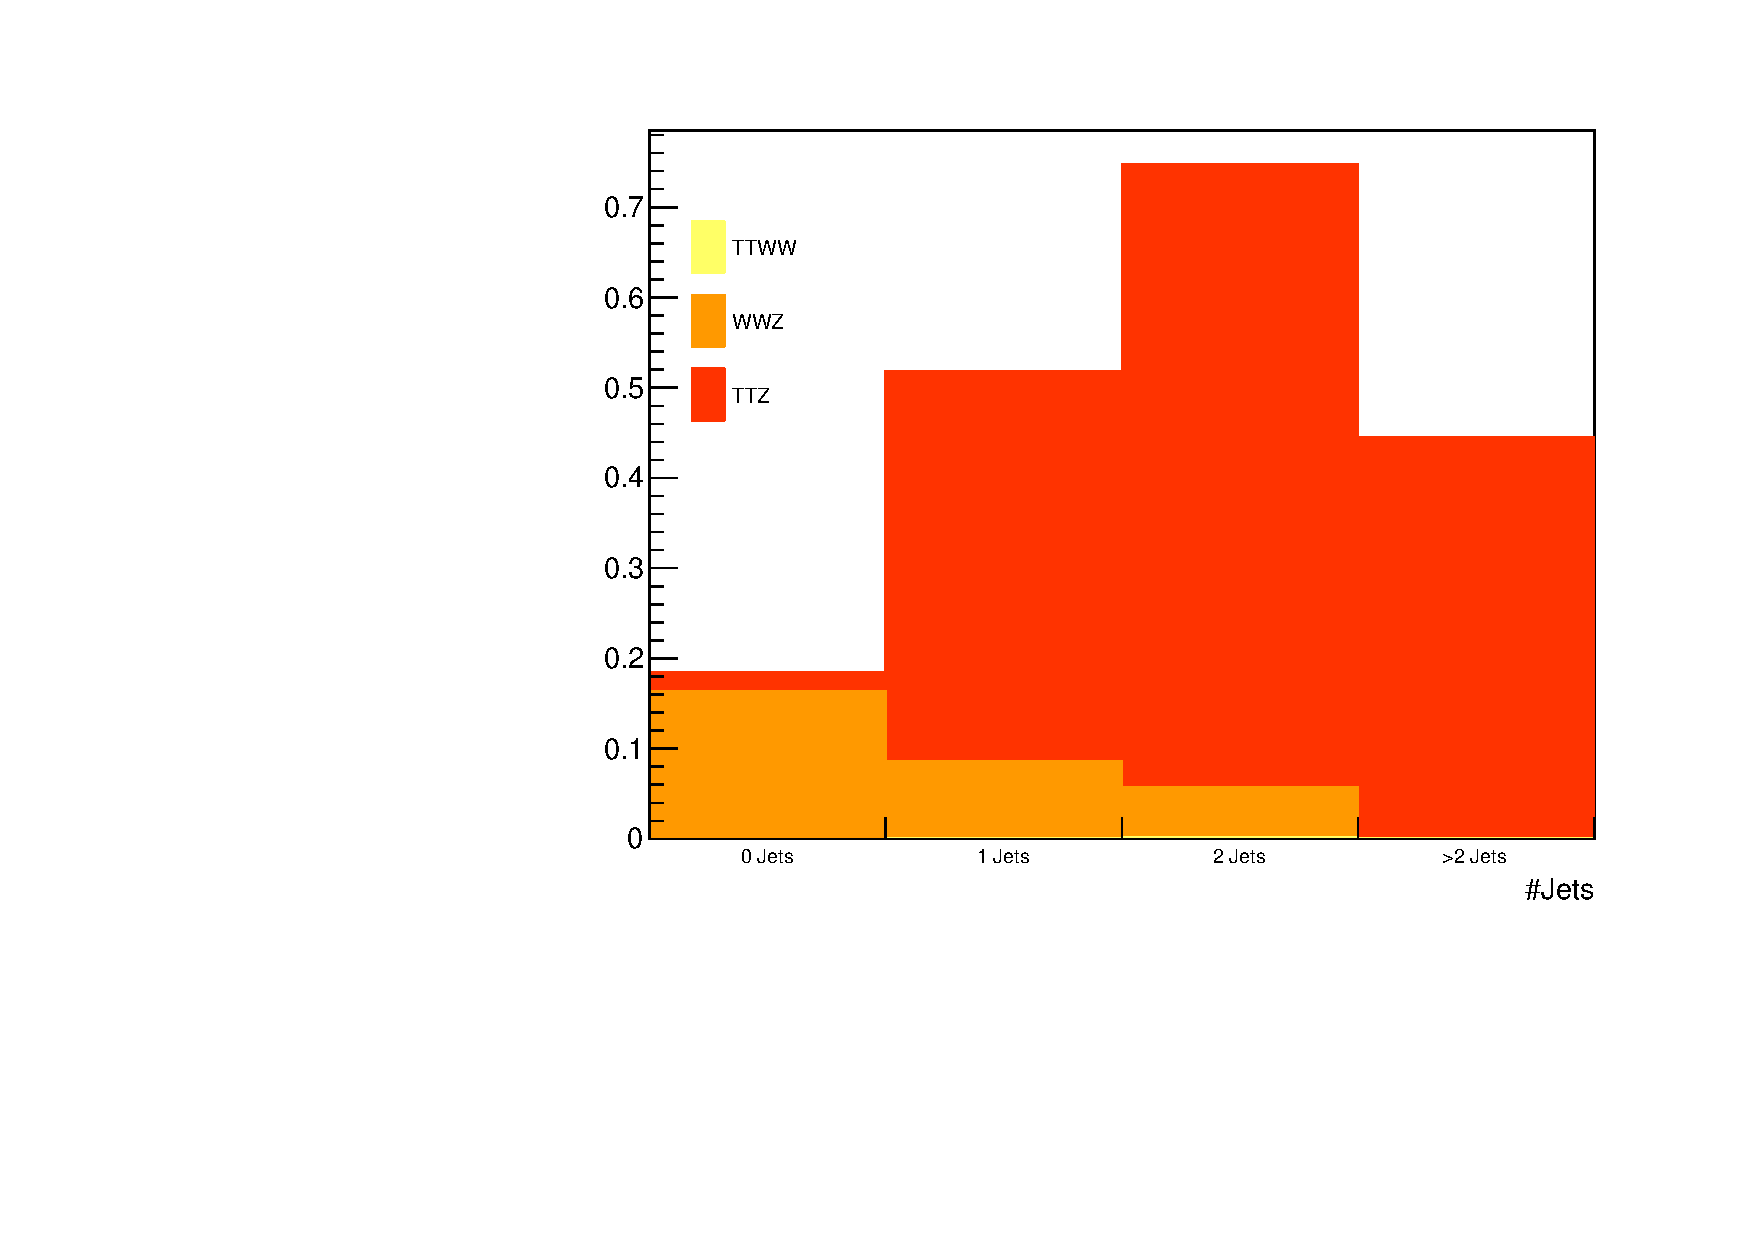
\includegraphics[width=\cmsFigWidth]{Figures/Jets_Irreducible_Bkg_MadGraphSet}
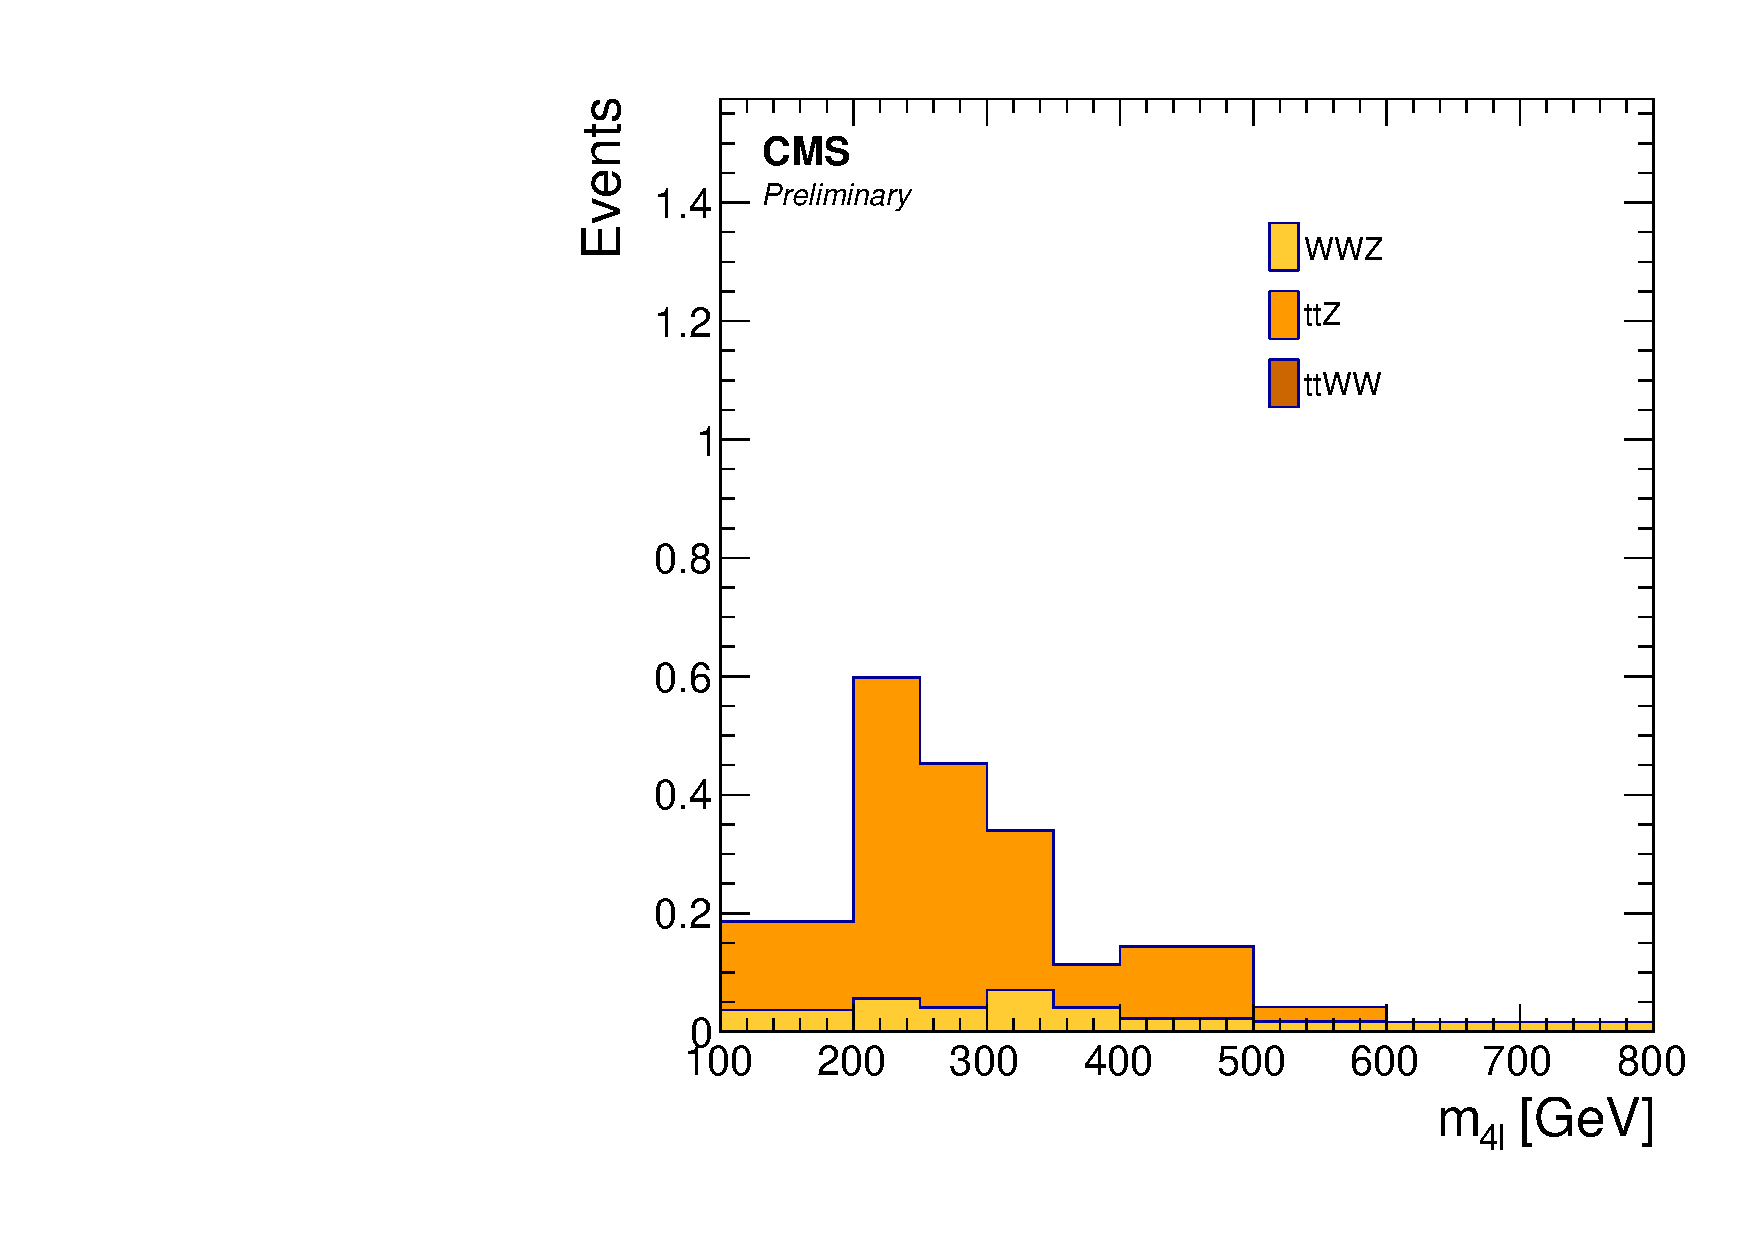
\includegraphics[width=\cmsFigWidth]{Figures/Mass_irr}
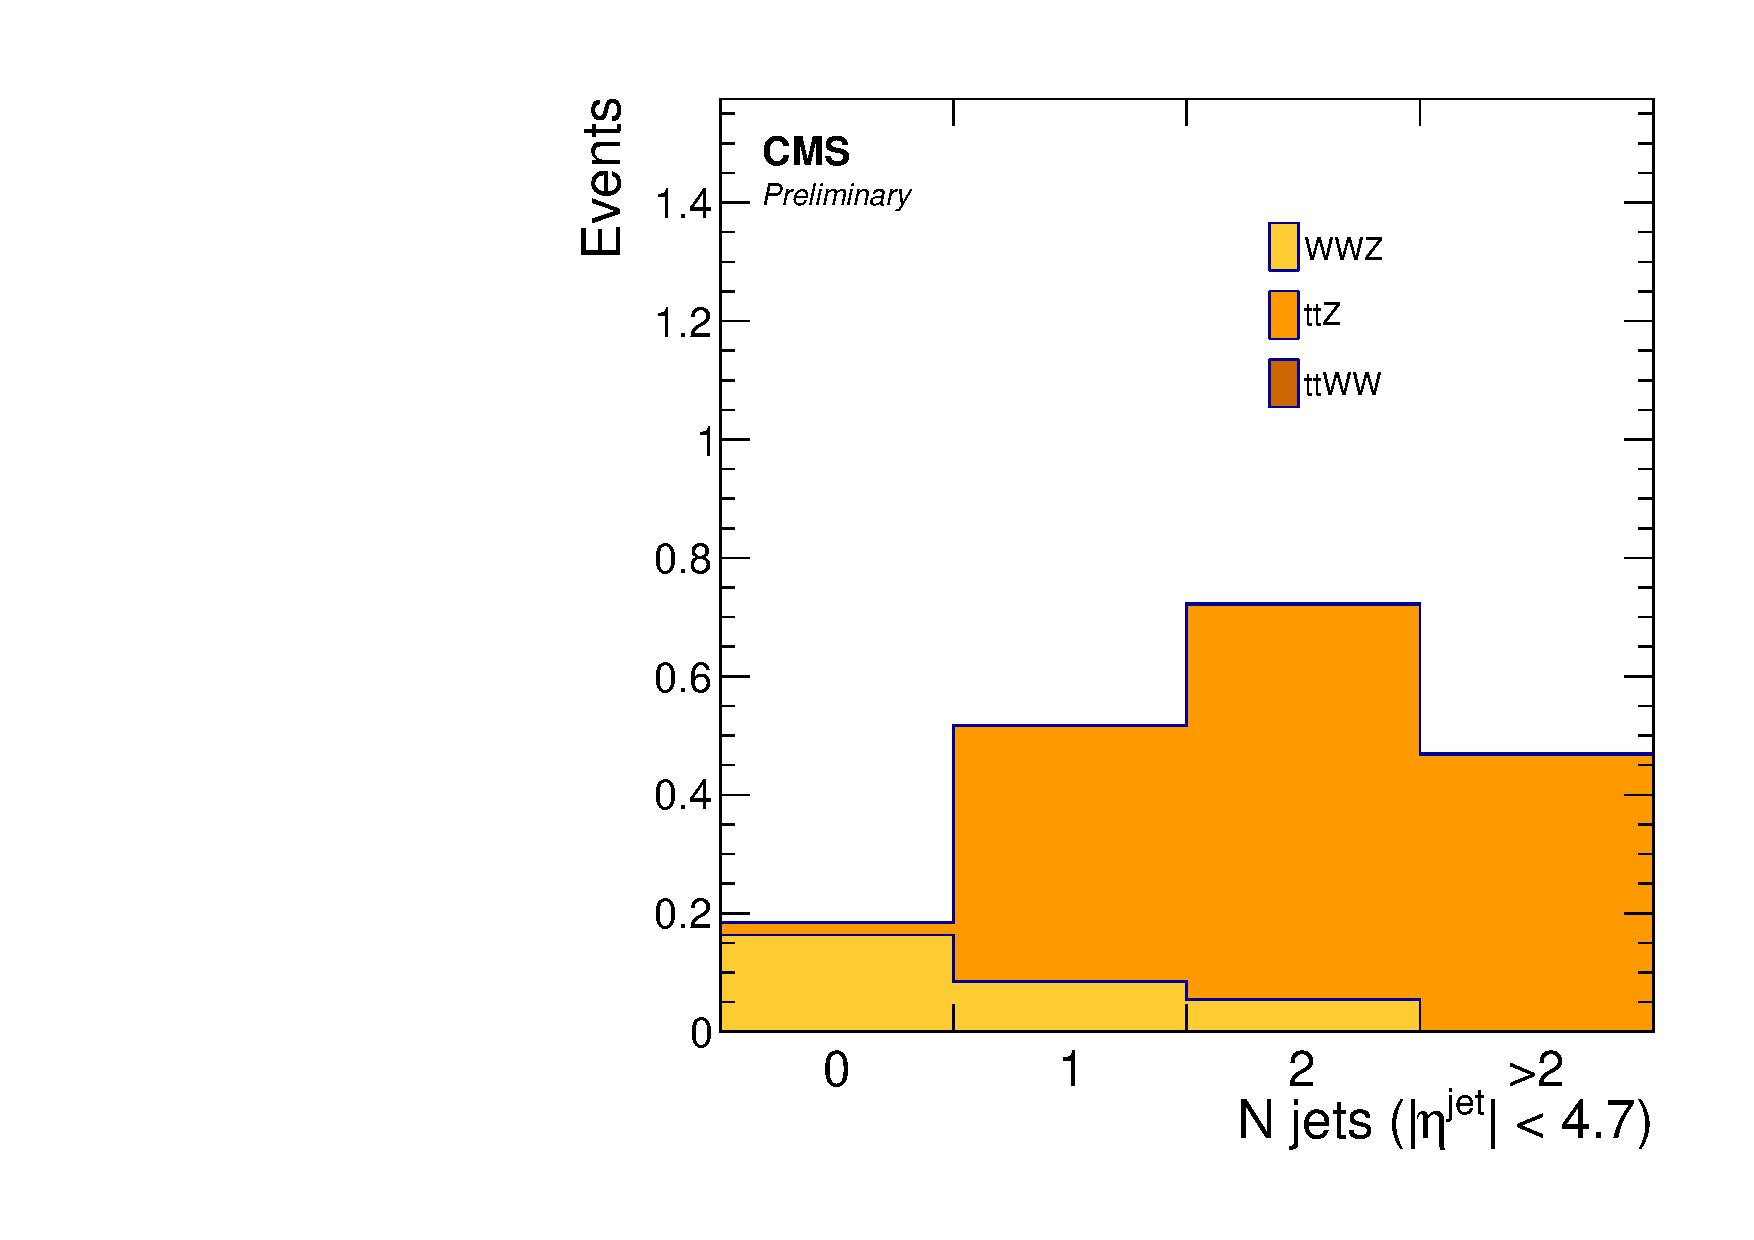
\includegraphics[width=\cmsFigWidth]{Figures/Jets_irr}
     \caption{Number of events of the irreducible background component in the signal region as a function of the invariant mass of the 4 lepton system (\cmsLeft) and the reconstructed number of jets produced in the event (\cmsRight).}
    \label{fig:irr_bkg}
  \end{center}
\end{figure}

The main background contribution that arises mostly from the $Z$ in association with jets, as well as from $t\bar{t}$, $WZ$ and
$WWW$ +jets, is estimated with data analyzed in dedicated control regions.
For this type of background, a jet or a non-prompt lepton (i.e. lepton produced in heavy meson decays) is misidentified as an isolated 
electron or muon. These processes are referred to as reducible background and are estimated using a data driven method, known
as ``method A'' in the $H\to ZZ \to 4\ell$ analysis~\cite{HiggsLegacyPaper}. This method is based on two control samples, obtained 
as subsets of four lepton events, by demanding a Z$_1$ candidate reconstructed with the same requirement as the  Z$_1$ built in the signal region, and two additional leptons, with opposite sign and same flavor ($e^\pm e^\mp$ or $\mu^\pm\mu^\mp$). The ``3P1F'' control sample contains events with only one of the two additional leptons failing identification and isolation 
criteria, the other being a good quality lepton, and it is used to estimate the contribution in the signal region of events with three genuine leptons, such as 
$WZ +$ jets.
In the ``2P2F'' control region, instead, the two additional leptons  are  both required  to  fail the final identification and isolation criteria. This  sample  is  meant  to  be  used  to  estimate  
both the  contribution  in  the  signal region and in the ``3P1F'' region of events with only two genuine leptons, such as Z + jets and $t\bar{t}$.  
The number of reducible background events in the signal region is given by the following formula:
\begin{equation}
\label{eq:redBkg_methA}
N^{red\ bkg}_{exp} = \sum_{i}^{N_{3P1F}} p_{i}- \sum_{i}^{N_{2P2F}} p_{i,1} p_{i,2},  
\end{equation}
where:
\begin{itemize}
\item $N_{3P1F}$ and $N_{2P2F}$ are the number of events in the ``3P1F'' and ``2P2F'' control regions respectively
\item $p_{i} = \frac{f_{i}}{1-f_{i}}$
\item $p_{i,1(2)} = \frac{f_{i,1(2)}}{1-f_{i,1(2)}}$
\item $f_{i}$  and $f_{i,1(2)}$ are the fake rates of the failing lepton in the ``3P1F'' sample and of the first (second) failing lepton in the ``2P2F'' control sample. 
\end{itemize}
The ``fake rate'' is the lepton misidentification probability $f(\pt^{\ell},\eta^{\ell})$
to extrapolate the background yields from the control region to the signal region. 
This probability is defined as the fraction of non-signal leptons passing the lepton selection of the analysis.
The fake rate is estimated in a sample composed by $Z_1 + 1\ell _{loose}$ events, 
where beside to the opposite sign/same flavor pair which forms the $Z_{1}$, 
exactly one additional lepton is reconstructed fulfilling all the selection requirements, 
but for the identification and the isolation cuts.\\
The lepton misidentification probability ranges from 1\% to 15\% and has a mild dependence on the pseudorapidities for the 
electrons.\\
In order to obtain the reducible background contribution as a function of the analyzed variables, the number of events in the ``3P1F'' and  ``2P2F'' 
control regions is estimated in each bin of each distribution separately, it is multiplied by the corresponding fake rate (depending on leptons $p_T$ and $\eta$) and summed, according to~\ref{eq:redBkg_methA}. In order to be consistent with the signal region, reconstructed jets that overlap with the loose leptons in the CRs are removed. In Figure~\ref{fig:red_bkg} the contribution of the reducible background is reported as a function of the 4-lepton invariant mass and the jet multiplicity, and it is estimated both from MC samples and by 
using the ``fake-rate'' method. The lack of statistics makes the data-driven estimate necessary.

\begin{figure}[hbtp]
  \begin{center}
   % 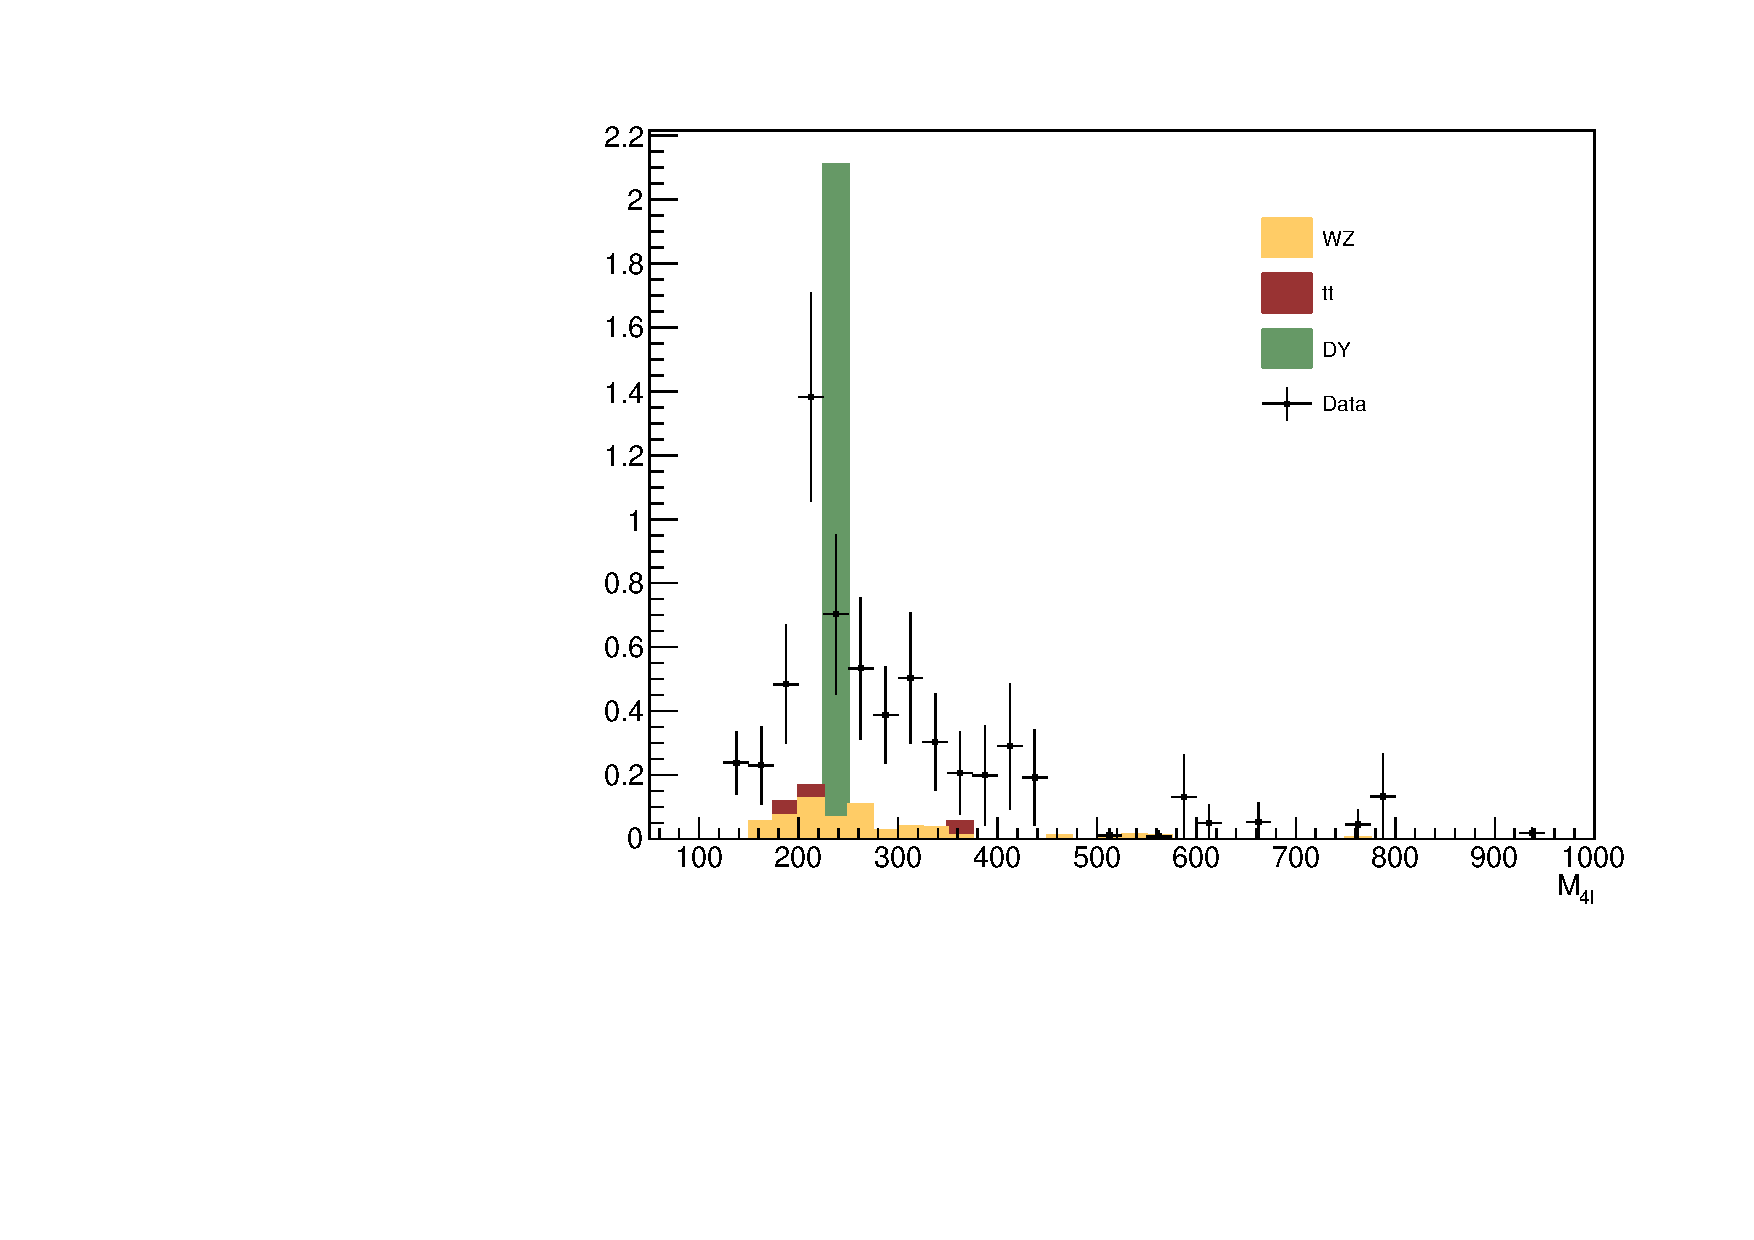
\includegraphics[width=\cmsFigWidth]{Figures/Mass_Reducible_Bkg_MadGraphSet}
    %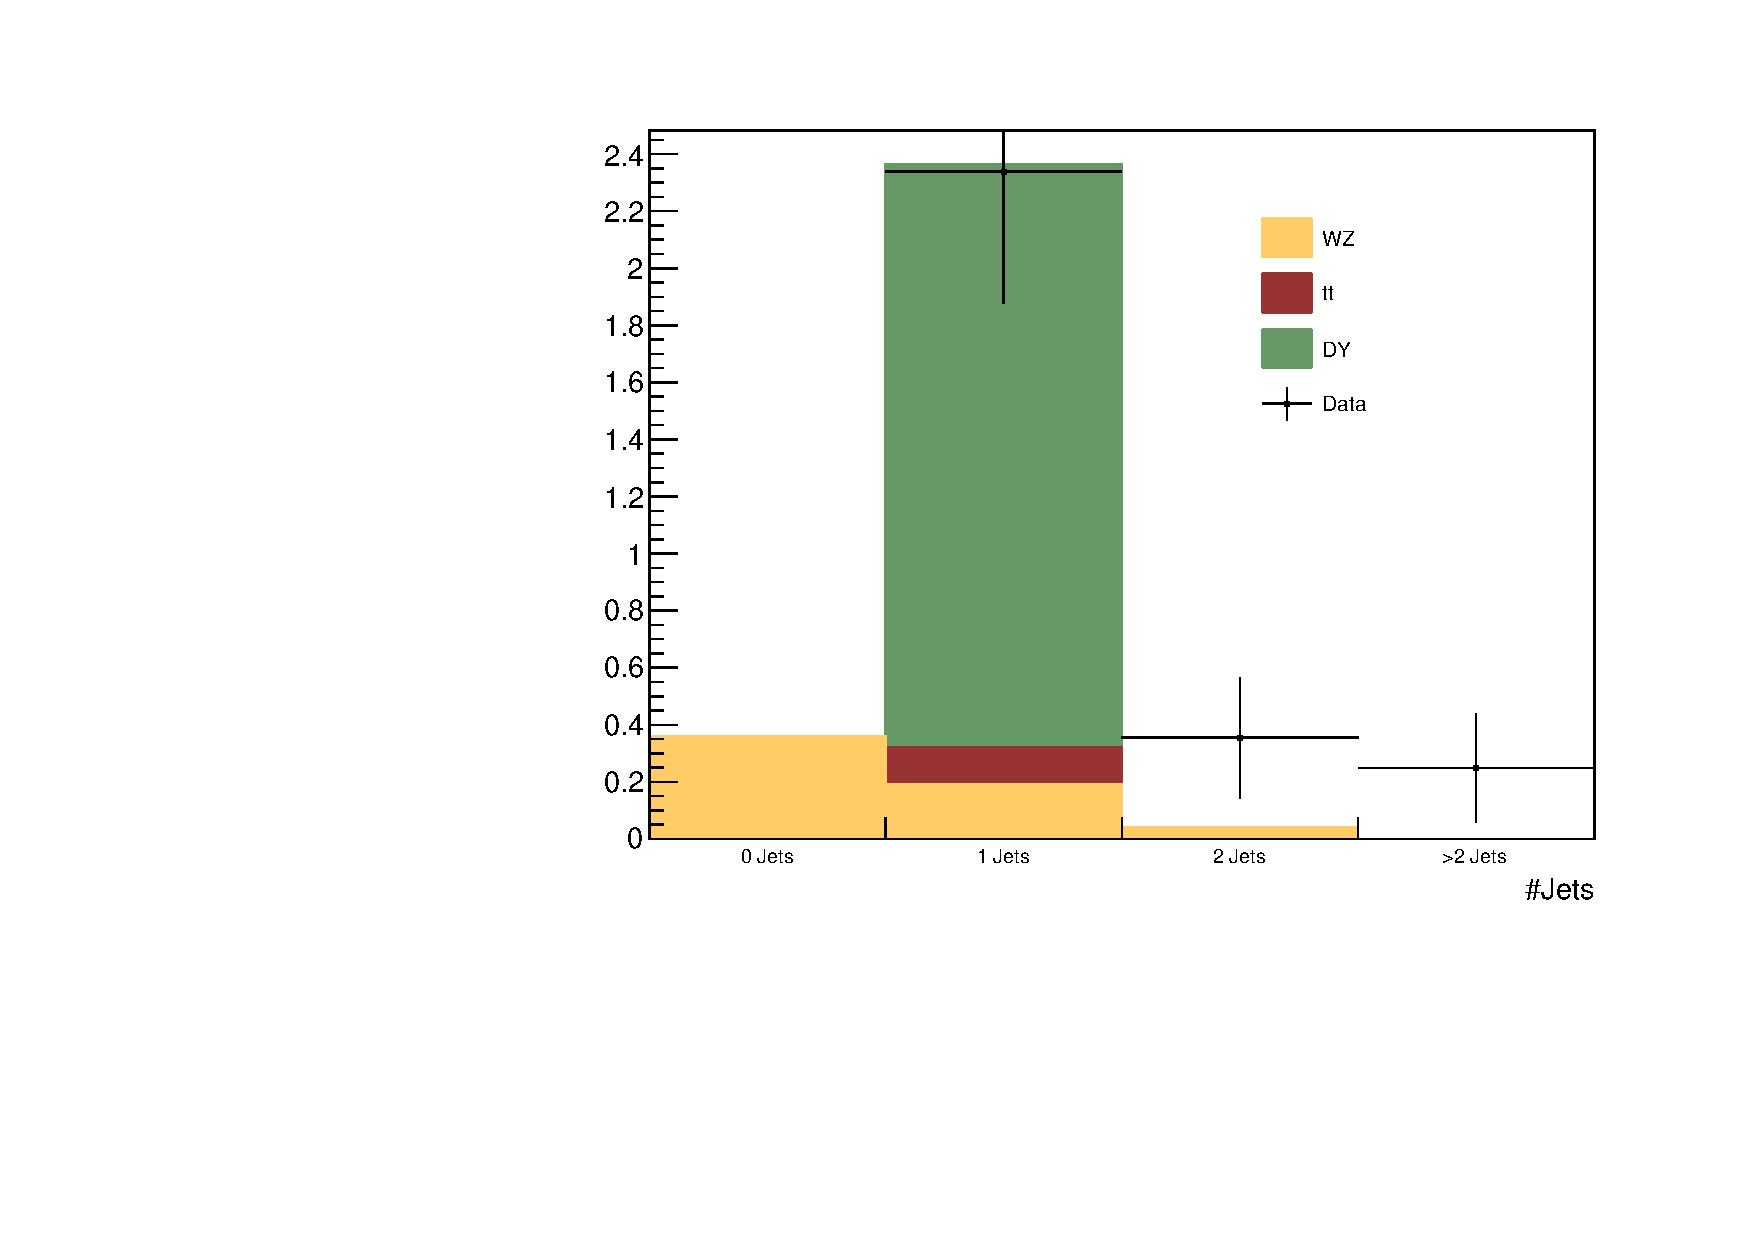
\includegraphics[width=\cmsFigWidth]{Figures/Jets_Reducible_Bkg_MadGraphSet}%FIXME 
    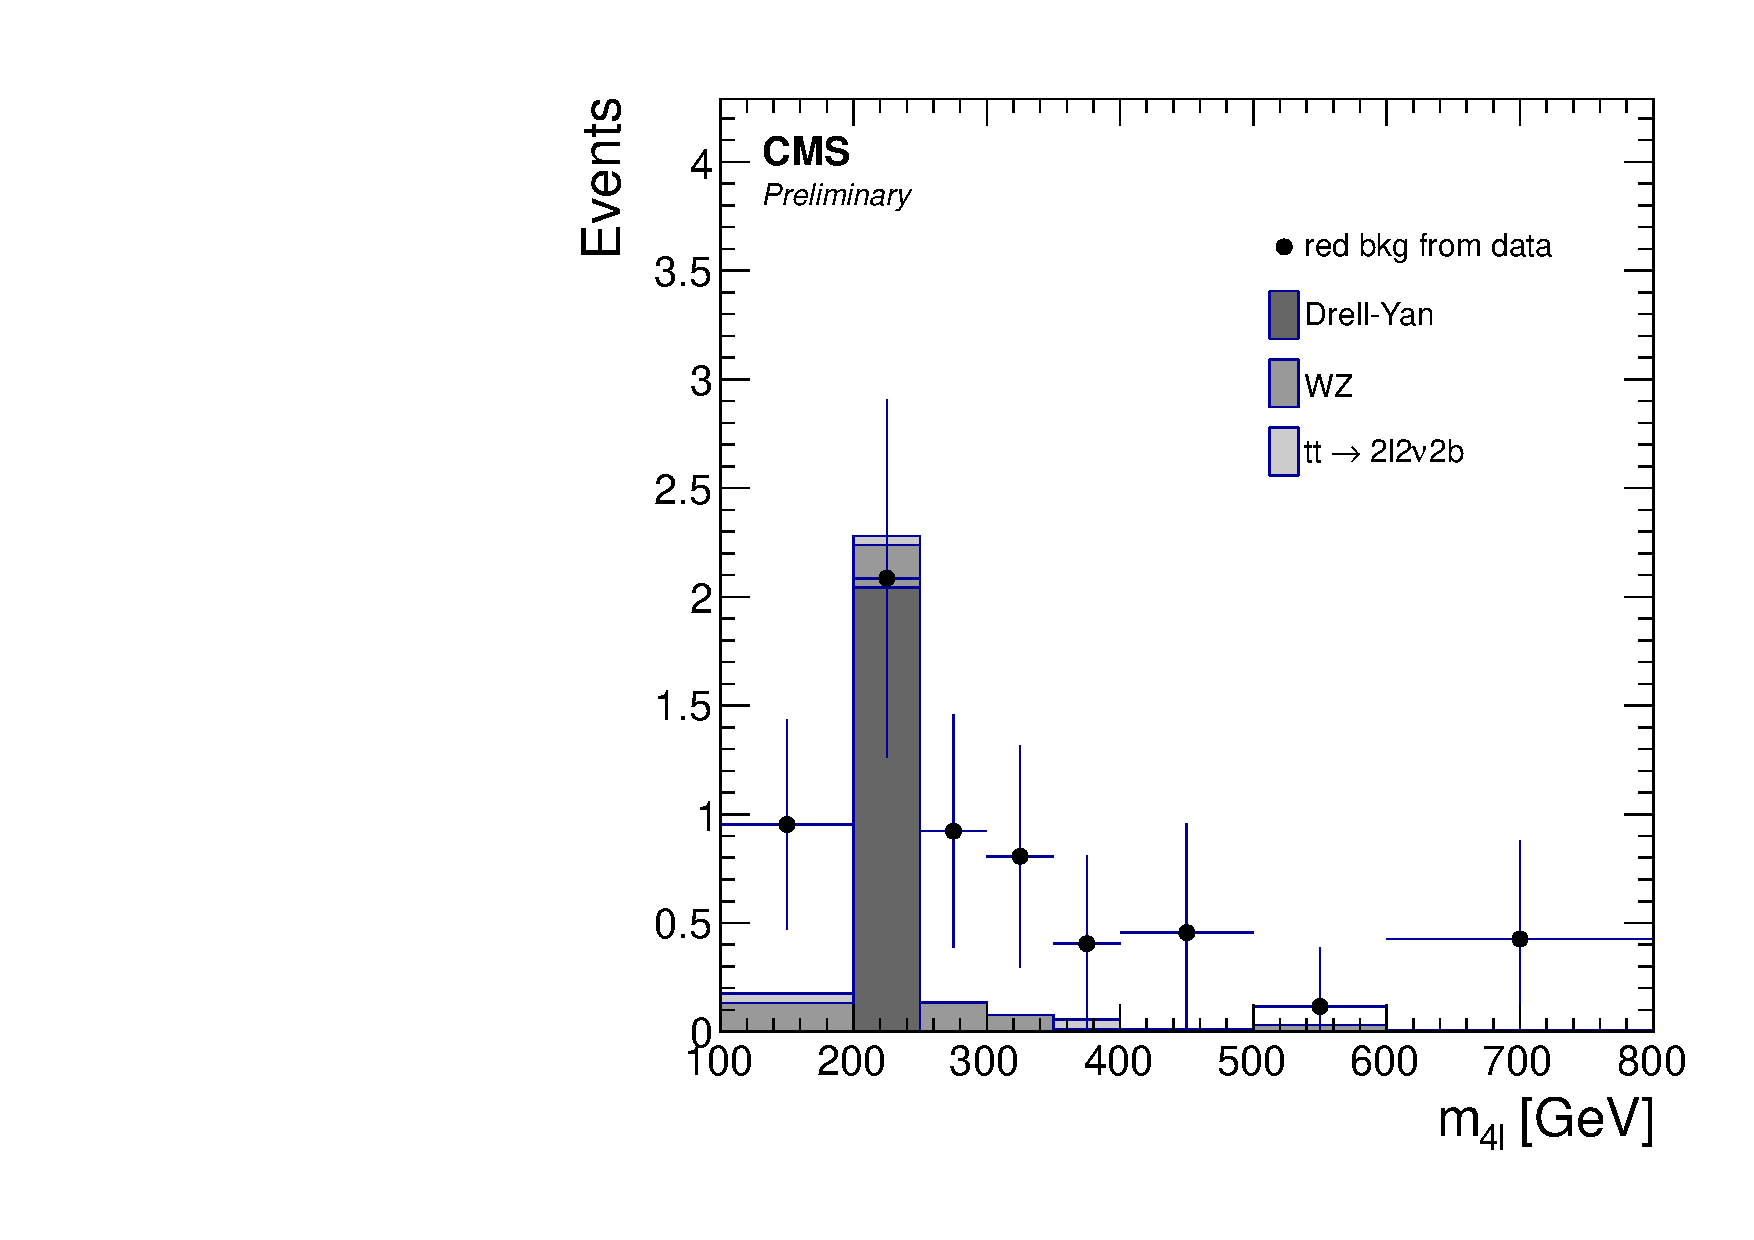
\includegraphics[width=\cmsFigWidth]{Figures/Mass_red}
    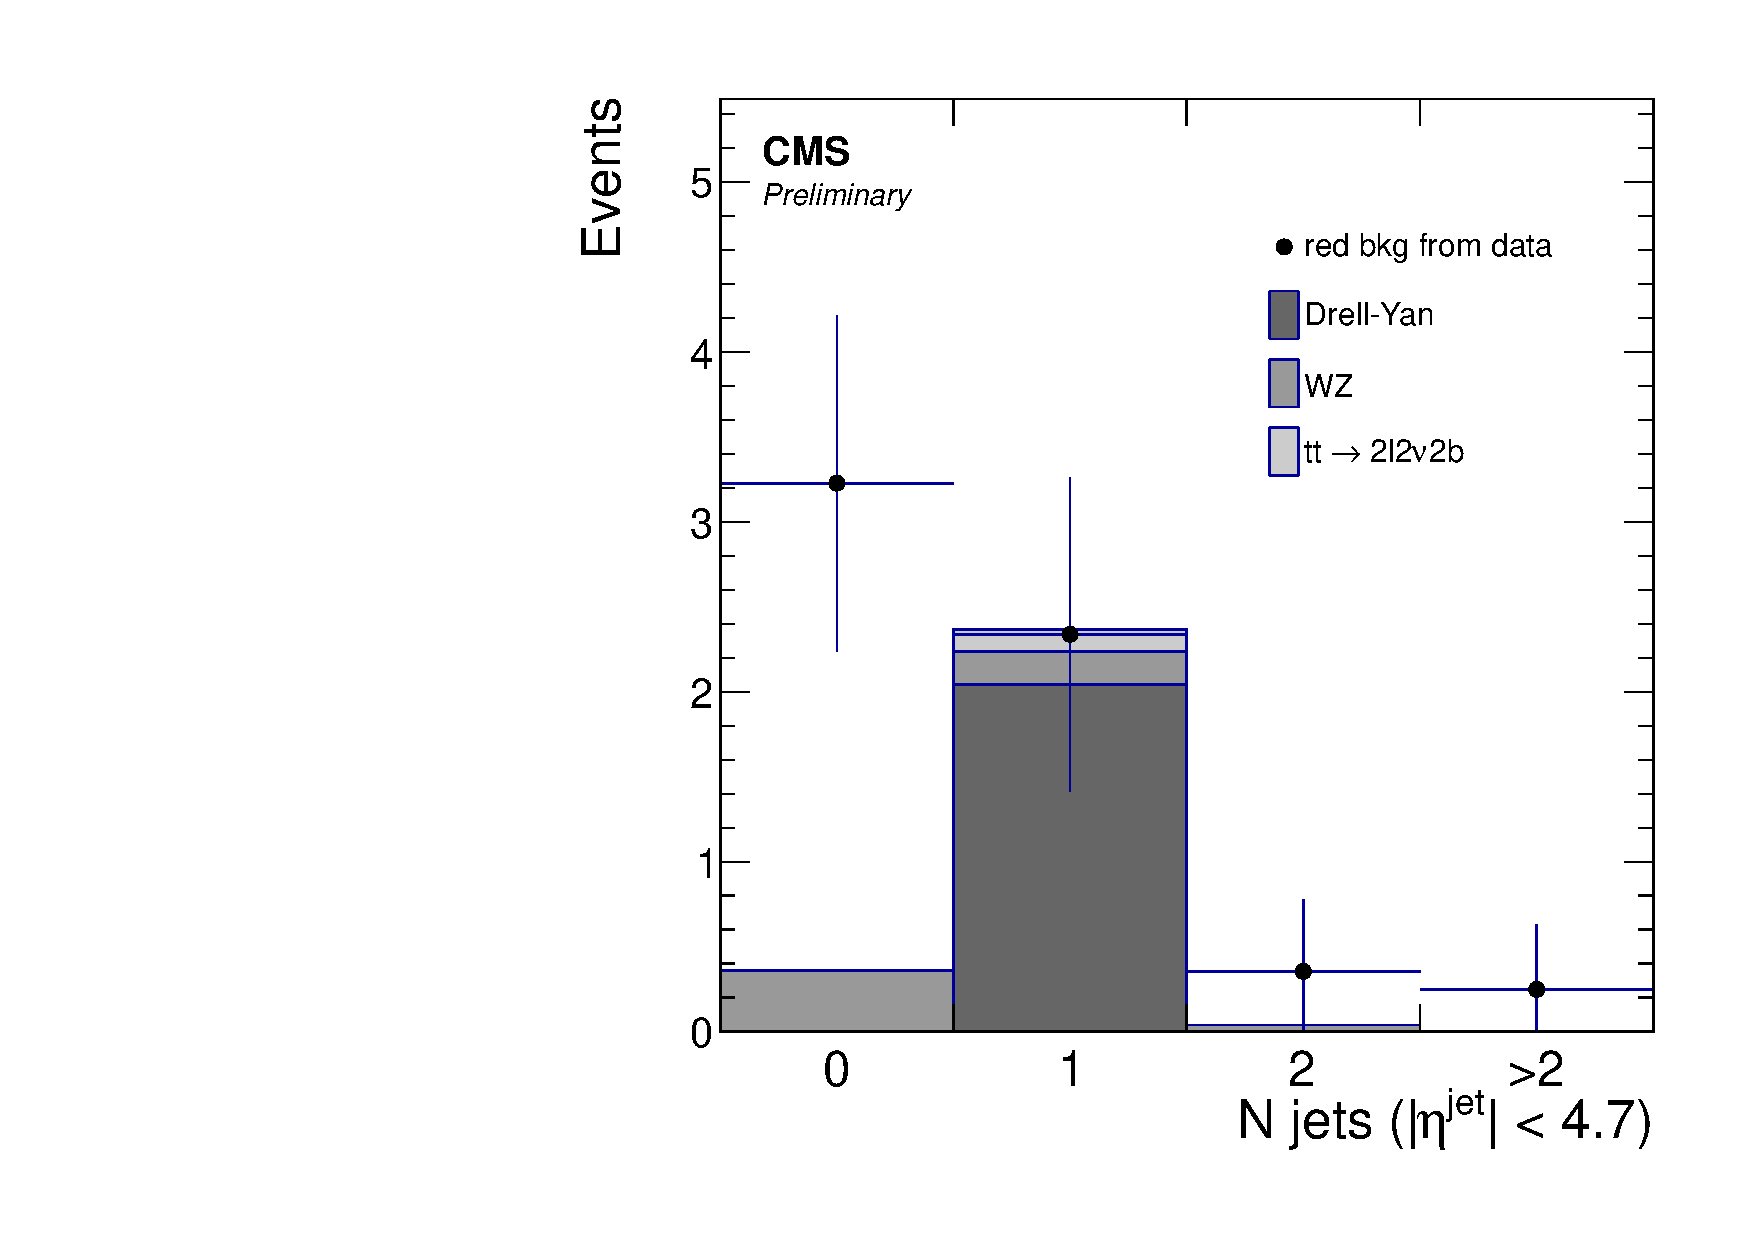
\includegraphics[width=\cmsFigWidth]{Figures/Jets_red}
     \caption{Reducible background component in the signal region as a function of the invariant mass of the 4 lepton system (\cmsLeft) and the reconstructed number of jets produced in the event (\cmsRight). Points represent the data-driven estimate, the stacked histogram represents the Monte Carlo predictions, characterized by a very poor statistics.}
    \label{fig:red_bkg}
  \end{center}
\end{figure}
%The reconstructed four-lepton invariant mass and the number of jets distributions are shown in Fig.~\ref{fig:sig_contr_Mad}.\\
%\begin{figure}[hbtp]
 % \begin{center}
  %  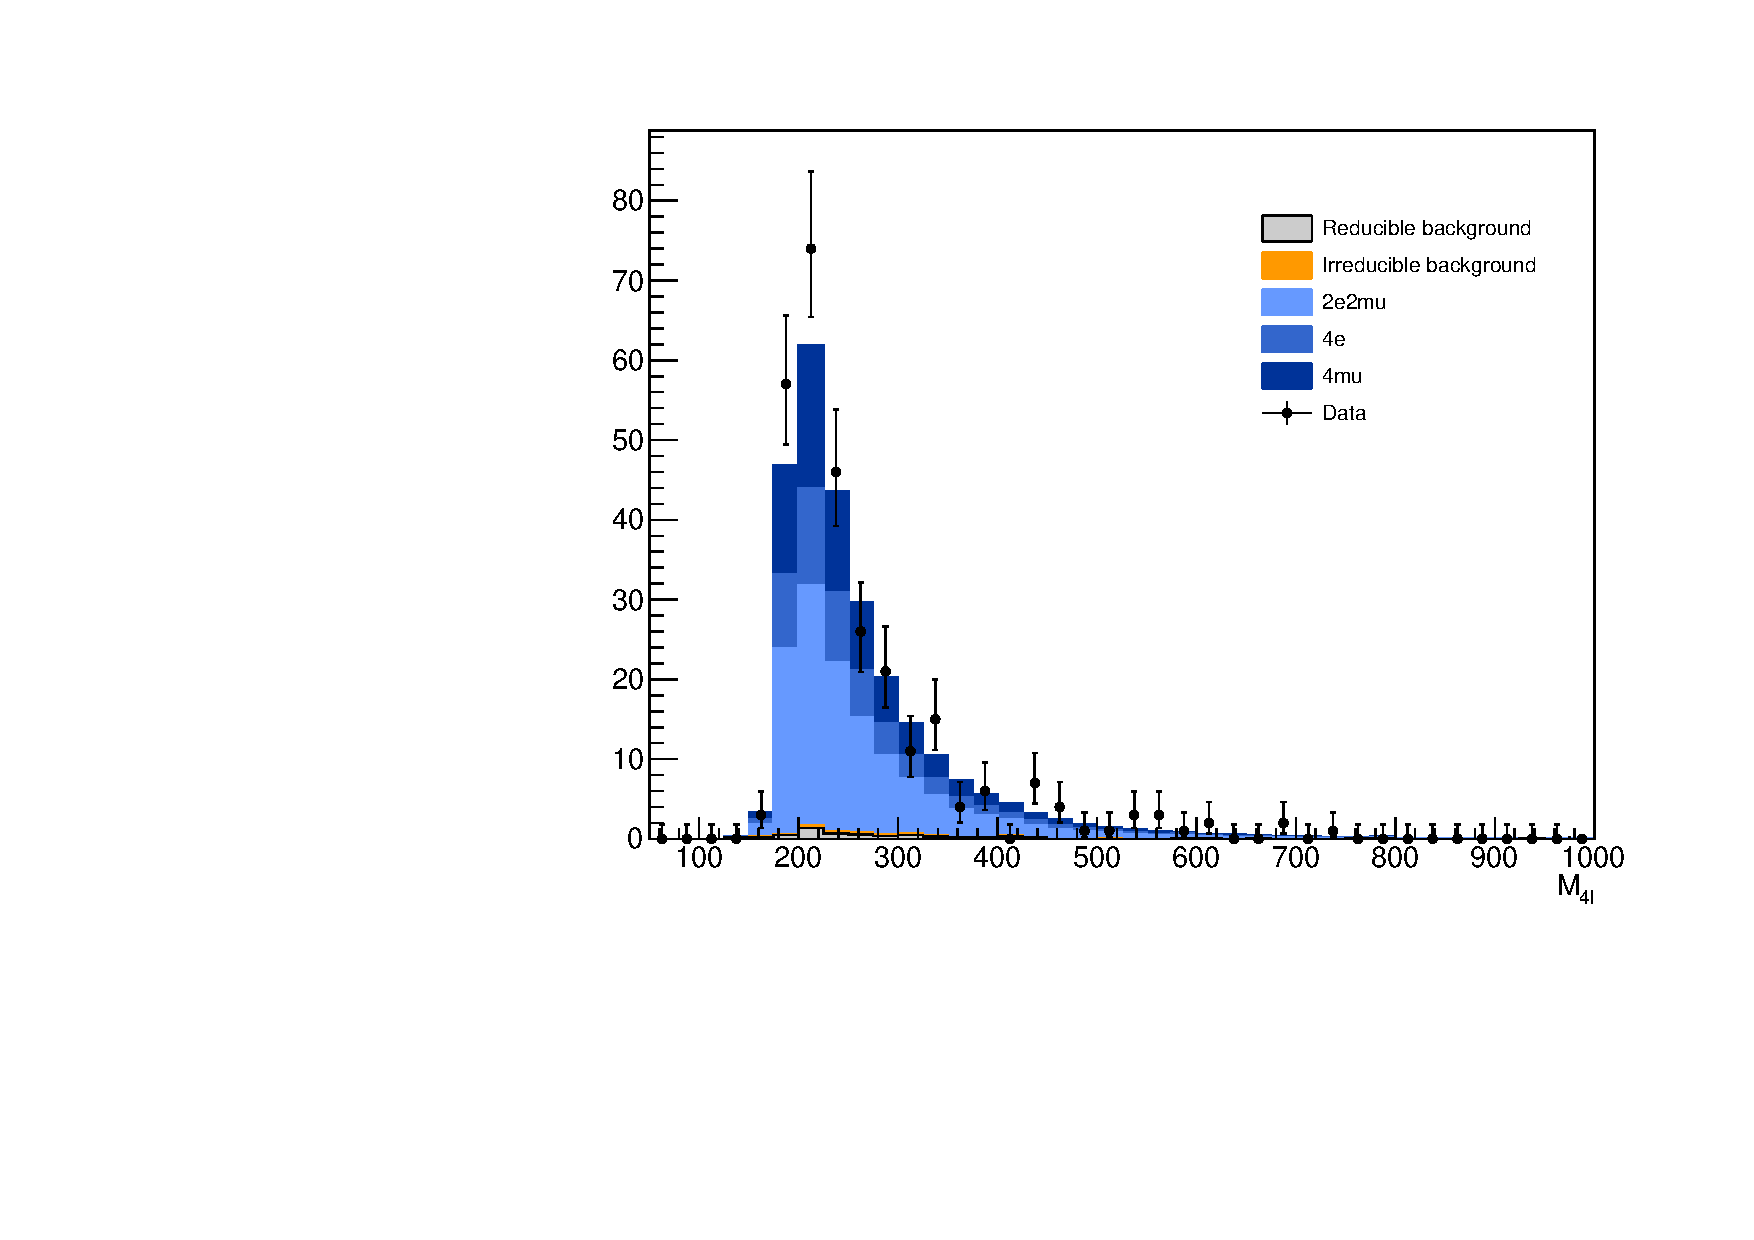
\includegraphics[width=\cmsFigWidth]{Figures/Mass_Final_State_MadGraphSet}
   % 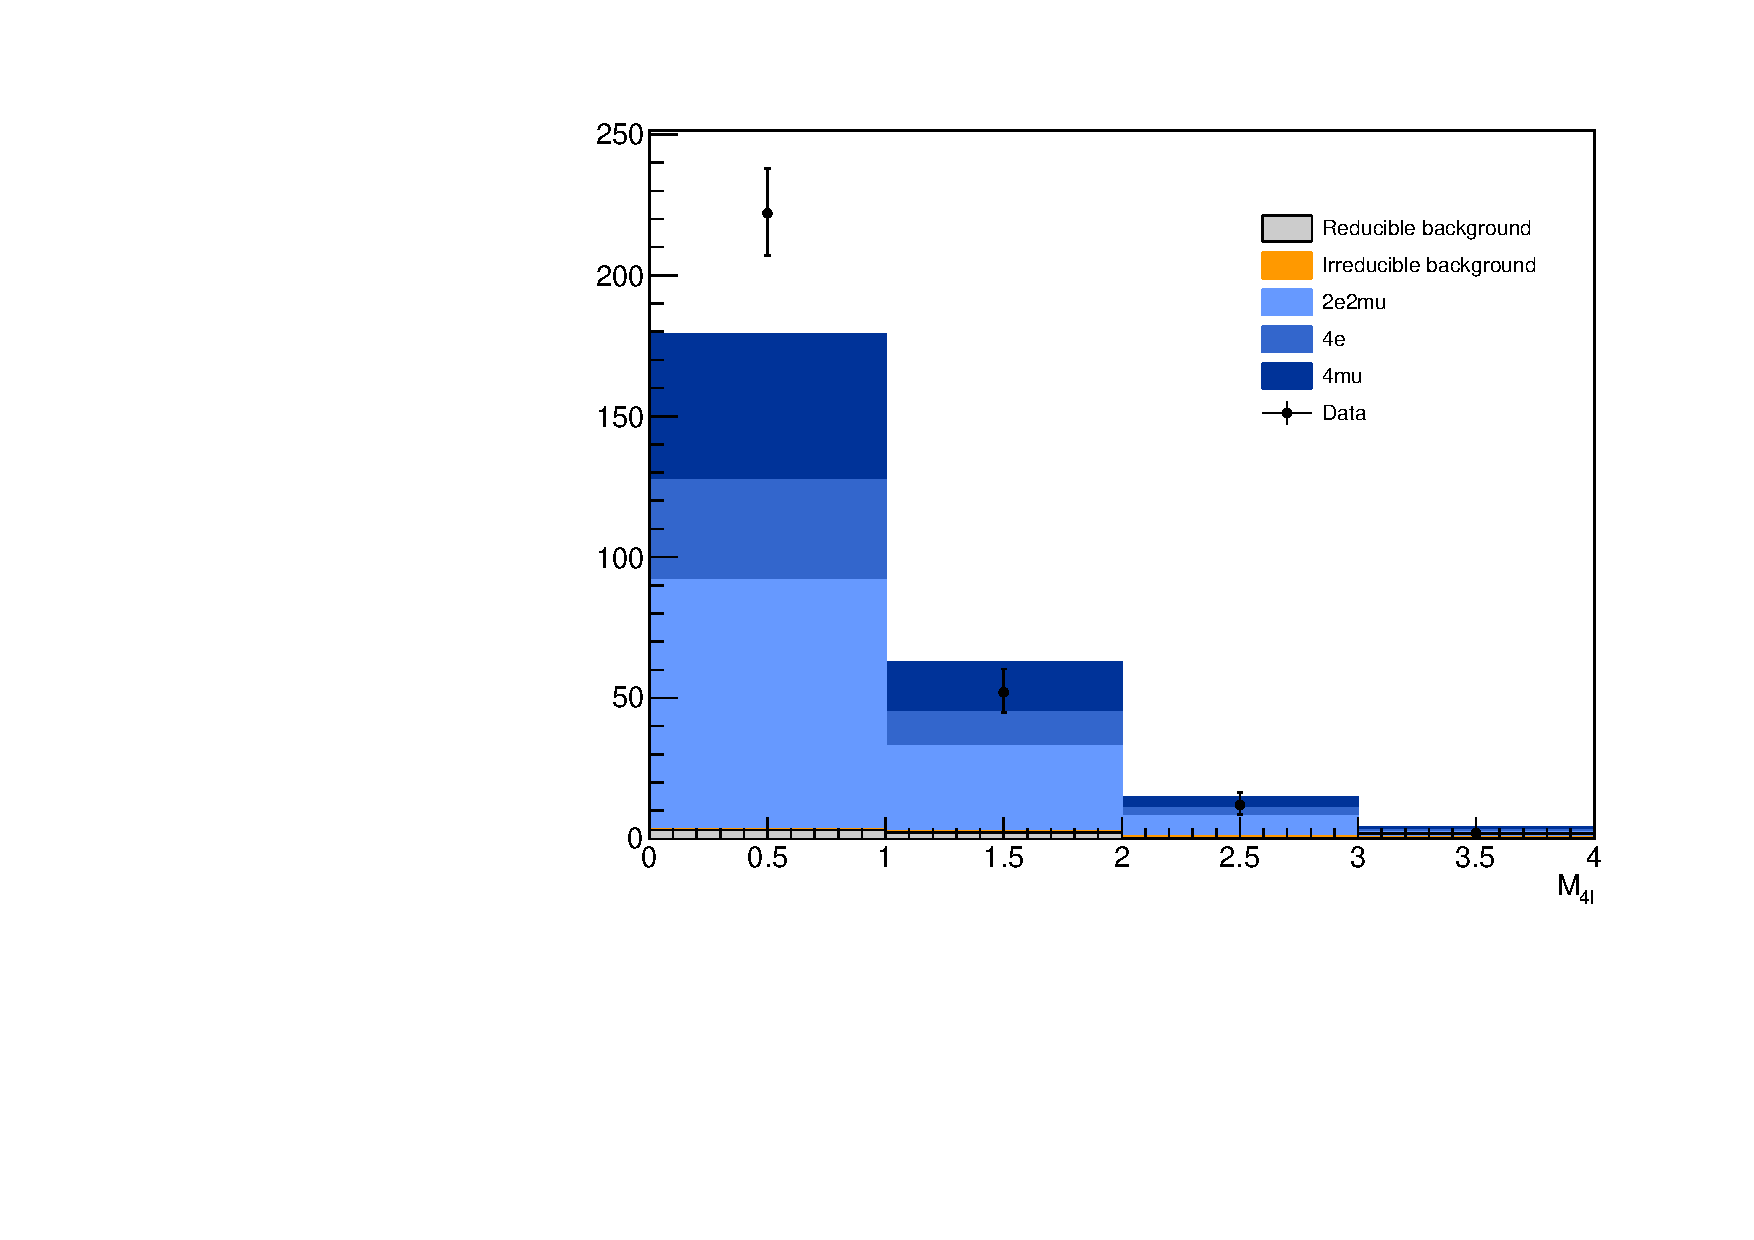
\includegraphics[width=\cmsFigWidth]{Figures/Jets_Final_State_MadGraphSet}
    % \caption{ Distribution of the reconstructed four-lepton mass (\cmsLeft). Distribution of the reconstructed number of jets produced in the event  (\cmsRight). Points represent the data, the stacked histogram represents the \texttt{MadGraph+MCFM+Phantom} predictions for $ZZ$ signal. The estimate of irreducible and reducible backgrounds is also reported.}
   % \label{fig:sig_contr_Mad}
 % \end{center}
%\end{figure}
